\documentclass{article}
\usepackage{amsmath,amssymb,graphicx,subfig}
\newcommand{\norm}[1]{\Vert #1 \Vert}
\newtheorem{theorem}{Theorem}
\newtheorem{lemma}[theorem]{Lemma}
\newcommand{\Prob}{\text{Prob}}
\newcommand{\Int}{\text{Int}}
\begin{document}
\title{Gibbs measures and the Ising model}
\author{Jordan Bell}
\date{July 1, 2014}
\maketitle

Let $\Lambda$ be a finite subset of $\mathbb{Z}^2$ and let $\Lambda'=\mathbb{Z}^2 \setminus \Lambda$. Let $\sigma' \in \{-1,+1\}^{\Lambda'}$, a fixed configuration of spins
outside $\Lambda$. Let $\Omega=\{-1,+1\}^\Lambda$; $\Omega$ is the space of all configurations of spins on $\Lambda$. We define a Hamiltonian $H_\Lambda(\cdot| \sigma') : \Omega \to \mathbb{R}$ (depending on the fixed external configuration $\sigma'$) by
\[
H_\Lambda(\sigma | \sigma')=-\sum_{\stackrel{x,y \in \Lambda}{|x-y|=1}} \sigma(x)\sigma(y)-\sum_{\stackrel{x \in \Lambda, y \in \Lambda'}{|x-y|=1}} \sigma(x) \sigma'(y).
\]
$H_\Lambda(\cdot | \sigma')$ gives the energy of a configuration $\sigma \in \Omega$, conditioned on the external configuration $\sigma'$.

For a parameter $\beta>0$ (called the {\em inverse temperature}), we define the {\em partition function} by
\[
Z(\beta,\Lambda,\sigma')=\sum_{\sigma \in \Omega} \exp(-\beta H_\Lambda(\sigma|\sigma')).
\]
Then we define the {\em Gibbs distribution} for the configuration space $\Omega$, depending on the external configuration $\sigma'$, by
\[
P_{\beta,\Lambda}(\sigma|\sigma')=\frac{1}{Z(\beta,\Lambda,\sigma')} \exp(-\beta H(\sigma|\sigma')).
\]
The purpose of the partition function is to normalize the above expression to be a probability measure on the configuration space $\Omega$.

For example, let $\Lambda$ be a square of side length $3$ centred at the origin, and take $\sigma'$ to be an external configuration of all negative spins. Define $\sigma \in \Omega$ by
\[
\begin{array}{lll}
\sigma(-1,1)=+1& \sigma(0,1)=+1 & \sigma(1,1)=-1\\
\sigma(-1,0)=-1 & \sigma(0,0)=+1 & \sigma(1,0)=-1\\
\sigma(-1,-1)=-1 & \sigma(0,-1)=-1 & \sigma(1,-1)=+1.
\end{array}
\]
We show this configuration in Figure \ref{figure1}. We calculate that the energy of this configuration is $H_\Lambda(\sigma|\sigma')=0$. We can calculate the energy of this configuration in a different way, using line segments separating lattice points with different spins, as follows. For an $n \times n$ square, there are $2n(n+1)$ nearest neighbor interactions. Put a line segment between every two 
lattice points with different spins; let $B(\sigma|\sigma')$ be the set of these line segments. We show this in Figure \ref{figure2}.




\begin{figure}
\begin{center}
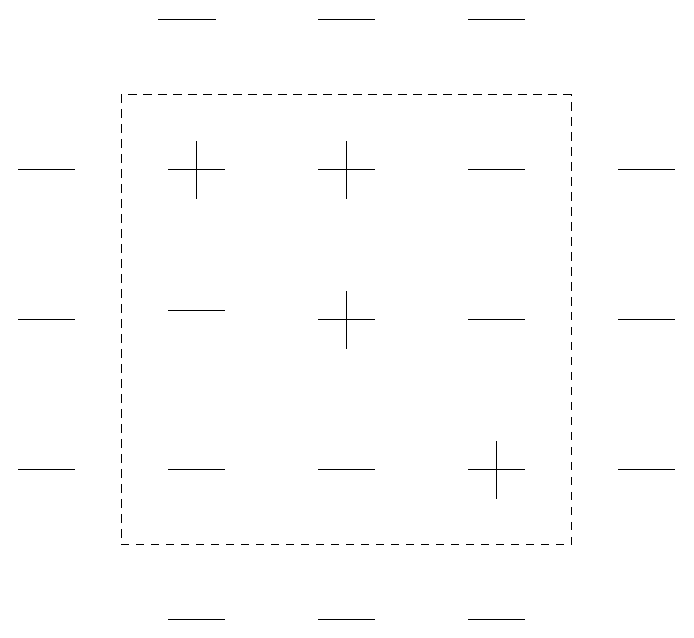
\includegraphics[width=0.5\textwidth]{config1}
\end{center}
\caption{An example of a configuration (and negative external spins)}
\label{figure1}
\end{figure}


\begin{figure}
\begin{center}
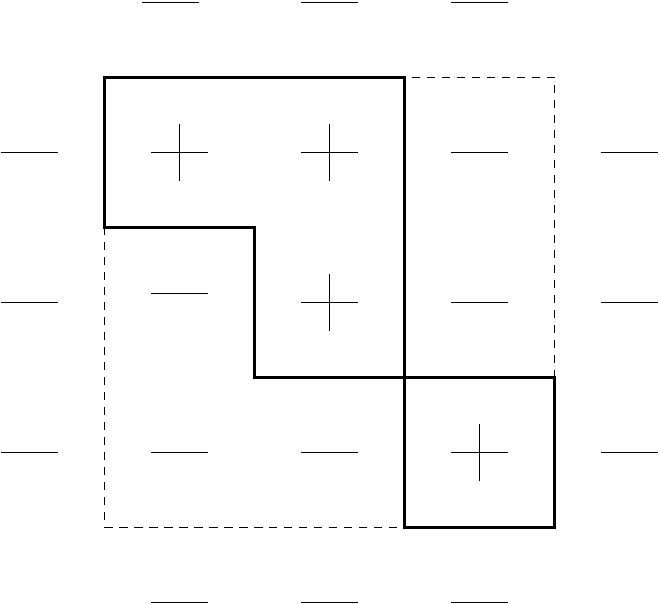
\includegraphics[width=0.5\textwidth]{config2}
\end{center}
\caption{Calculating energy using contours}
\label{figure2}
\end{figure}

Generally, if $\Lambda$ is an $n \times n$ square then we have
\[
H_\Lambda(\sigma|\sigma')=-2n(n+1)+2|B(\sigma|\sigma')|.
\]
Indeed, in our above example, $n=3$ and $|B(\sigma|\sigma')|=12$, so the above expression is $-24+2\cdot 12=0$, and we have already calculated that $H_\Lambda(\sigma|\sigma')=0$. What matters is that if we know the external configuration, then to describe the configuration inside a region $\Lambda$ it suffices to know the edges that separate opposite spins. And since the energy of any configuration has the term $-2n(n+1)$ and this appears in the numerator and denominator of the expression for the Gibbs distribution, we can omit it to calculate the Gibbs distribution. By a {\em contour} we mean a closed path of edges that does not intersect itself. We can express the Gibbs distribution in terms of contours as
\[
P_{\beta,\Lambda}(\sigma|\sigma')=\frac{\prod_{\gamma \in \Gamma(\sigma,\sigma')} \exp(-2|\gamma|)}{\sum_{\Gamma} \prod_{\gamma \in \Gamma} \exp(-2\beta|\gamma|)};
\]
$\Gamma(\sigma,\sigma')$ is the set of contours corresponding to the configuration $\sigma$ with the external configuration $\sigma'$, and the summation is over all sets $\Gamma$ of nonintersecting contours. 

We are not in fact interested in the Gibbs distribution on the configurations on a finite subset $\Lambda$ of $\mathbb{Z}^2$, but instead limits of Gibbs distributions with
$\Lambda_n \to \mathbb{Z}^2$. A Gibbs distribution $P_{\beta,\Lambda}(\cdot|\sigma')$ on $\Omega$ is in fact a probability measure on $\{+1,-1\}^{\mathbb{Z}^2}$: for $\sigma \in
\{+1,-1\}^{\mathbb{Z}^2}$, a configuration on the plane, we define
\[
\widetilde{P}_{\beta,\Lambda}(\sigma|\sigma')=\begin{cases}
0&\sigma|\Lambda' \neq \sigma'\\
P_{\beta,\Lambda}((\sigma|\Lambda) |\sigma')&\sigma|\Lambda'=\sigma'.
\end{cases}
\]

Fix some $\beta$.
Let $\Lambda_n$ be a sequence of $n \times n$ squares centred at the origin, let $\sigma_{n,+}'$ be a sequence of external configurations where all lattice points outside $\Lambda_n$
have positive spins, and let $\sigma_{n,-}'$ be a sequence of external configurations where all lattice points outside $\Lambda_n$ have negative spins.
Let $P_{n,+}$ be the sequence of Gibbs distributions corresponding to the positive external spins, and let $P_{n,-}$ be the sequence of Gibbs distributions corresponding to the negative external spins. These extend to probability measures $\widetilde{P}_{n,+}$ and $\widetilde{P}_{n,-}$ on $\{+1,-1\}^{\mathbb{Z}^2}$. Since $\{+1,-1\}$ is a compact metrizable space, the product $\{+1,-1\}^{\mathbb{Z}^2}$ is a compact metrizable space and thus the space of probability measures on it is compact. Hence the sequence $\widetilde{P}_{n,+}$
has at least one limit point, say $P_{+}$, and the sequence $\widetilde{P}_{n,-}$ has at least one limit point, say $P_{-}$. We shall show that $P_+ \neq P_-$, namely that there is not a unique limit Gibbs measure on the set of all configurations on $\mathbb{Z}^2$.


Let $V_+=\{\sigma \in \{+1,-1\}^{\mathbb{Z}^2}: \sigma(0)=+1\}$ and $V_-= \{\sigma \in \{+1,-1\}^{\mathbb{Z}^2}:\sigma(0)=-1\}$. Suppose that for all $n$ we had
$\widetilde{P}_{n,+}(V_-) < \frac{1}{3}$. Taking limits we have that $P_+(V_-) \leq \frac{1}{3}$ and so $P_+(V_+) \geq \frac{2}{3}$ (since the events $V_+$ and $V_-$ are disjoint and their union is the set of all configurations on $\mathbb{Z}^2$). But $\widetilde{P}_{n,+}(V_-)=\widetilde{P}_{n,-}(V_+)$, so taking limits we also get $P_-(V_+) \leq \frac{1}{3}$. Therefore the measures $P_+$ and $P_-$ give different measures to the set $V_+$, so they are distinct. Thus to show that the measures $P_+$ and $P_-$ are distinct it suffices to show that for all $n$ we have $\widetilde{P}_{n,+}(V_-) < \frac{1}{3}$.

We have
\begin{eqnarray*}
\widetilde{P}_{n,+}(V_-)&\leq&\Prob\left(\textrm{there exists a contour} \, \gamma \subset B(\sigma|\sigma'), 0 \in \Int(\gamma)\right)\\
&\leq&\sum_{\stackrel{\gamma}{0 \in \Int(\gamma)}} \Prob(\gamma \subset B(\sigma|\sigma'))\\
&\leq&\sum_{\stackrel{\gamma}{0 \in \Int(\gamma)}} \exp(-2\beta|\gamma|).
\end{eqnarray*}
The above sum is over all contours such that the origin lies in their interior. We can write the set of all contours around the origin as a union of the set of all contours of length $k$ around the origin, $k \geq 4$. There are at most $\left( \frac{k}{4} \right)^2 4^k$ contours of length $k$ around the origin. Therefore
\[
\widetilde{P}_{n,+}(V_-)\leq\sum_{k=4}^\infty \frac{k^2}{16} \cdot 4^k \exp(-2\beta k).
\]
As $\beta \to \infty$, this is $O(\exp(-8\beta))$. In particular there is some $\beta_0$ such that if $\beta \geq \beta_0$ then for all $n$ we have $\widetilde{P}_{n,+}(V_-)< \frac{1}{3}$. This shows
that the limit Gibbs measures gives different measures to the set $V_+$, hence they are distinct. 

\section*{Further reading}
Minlos \cite{minlos}, Sinai \cite{MR691854}, Cipra \cite{MR936054}, Simon \cite{simon},  Le Ny \cite{ny}, Kadanoff \cite{kadanoff}.

\bibliographystyle{plain}
\bibliography{ising}


\end{document}